\section{State Machines}

State machines consist of states, inputs, outputs,
and transition functions that determine how the
machine moves between states based on inputs.

A state machine can be defined mathematically as a 5-tuple $(Q, \Sigma, \delta, q_0, F)$ where:
\begin{itemize}
    \item $Q$ is a finite set of states
    \item $\Sigma$ is a finite set of input symbols
    \item $\delta: Q \times \Sigma \rightarrow Q$ is the transition function
    \item $q_0 \in Q$ is the initial state
    \item $F \subseteq Q$ is the set of final states
\end{itemize}

\begin{figure}[h]
    \centering
    \begin{tikzpicture}[node distance=3cm, on grid, auto]
        % States
        \node[state, initial] (q0) {$q_0$};
        \node[state] (q1) [right=of q0] {$q_1$};
        \node[state, accepting] (q2) [right=of q1] {$q_2$};

        % Transitions
        \path[->]
        (q0) edge [bend left=30] node {1} (q1)
        (q0) edge [loop below] node {0} ()
        (q1) edge [bend left=30] node {0} (q0)
        (q1) edge node {1} (q2)
        (q2) edge [loop below] node {0,1} ();
    \end{tikzpicture}
    \caption{A simple finite state machine with three states}
    \label{fig:basic_fsm}
\end{figure}

\subsection{Moore and Mealy Machines}

In digital design, state machines are typically categorized into two primary types: Moore machines and Mealy machines.

\subsection*{Moore Machines}

In a Moore machine, outputs depend solely on the current state. The output function can be defined as $\lambda: Q \rightarrow \Delta$, where $\Delta$ is the output alphabet. This makes Moore machines synchronous and deterministic, as outputs change only when the state changes at clock edges.

\begin{figure}[h]
    \centering
    \begin{tikzpicture}[node distance=3.5cm, on grid, auto]
        % Moore machine states with outputs inside nodes
        \node[state, initial] (A) {$A/0$};
        \node[state] (B) [right=of A] {$B/1$};

        % Transitions
        \path[->]
        (A) edge [bend left=20] node {1} (B)
        (A) edge [loop below] node {0} ()
        (B) edge [bend left=20] node {0} (A)
        (B) edge [loop below] node {1} ();
    \end{tikzpicture}
    \caption{Moore machine with outputs indicated in each state}
    \label{fig:moore_machine}
\end{figure}

\subsection*{Mealy Machines}

In a Mealy machine, outputs depend on both the current state and the current input. The output function is defined as $\lambda: Q \times \Sigma \rightarrow \Delta$. As a result, Mealy machines can change their outputs without changing states, providing faster response to inputs.

\begin{figure}[h]
    \centering
    \begin{tikzpicture}[node distance=3.5cm, on grid, auto]
        % Mealy machine states
        \node[state, initial] (A) {$A$};
        \node[state] (B) [right=of A] {$B$};

        % Transitions with input/output
        \path[->]
        (A) edge [bend left=25] node[sloped,pos=0.4] {1/1} (B)
        (A) edge [loop below] node {0/0} ()
        (B) edge [bend left=25] node[sloped,pos=0.4] {0/1} (A)
        (B) edge [loop below] node {1/0} ();
    \end{tikzpicture}
    \caption{Mealy machine with input/output pairs on transitions}
    \label{fig:mealy_machine}
\end{figure}

\subsection{State Encoding and Implementation}

State machines are implemented in hardware using memory elements (flip-flops) to store the current state and combinational logic to determine the next state and outputs. The process involves:

\begin{enumerate}
    \item Drawing the state diagram
    \item Creating a state transition table
    \item Encoding the states using flip-flops
    \item Deriving the next-state and output functions
    \item Implementing the design using logic gates and flip-flops
\end{enumerate}

The number of flip-flops required equals $\lceil \log_2 n \rceil$, where $n$ is the number of states.

\begin{figure}[h]
    \centering
    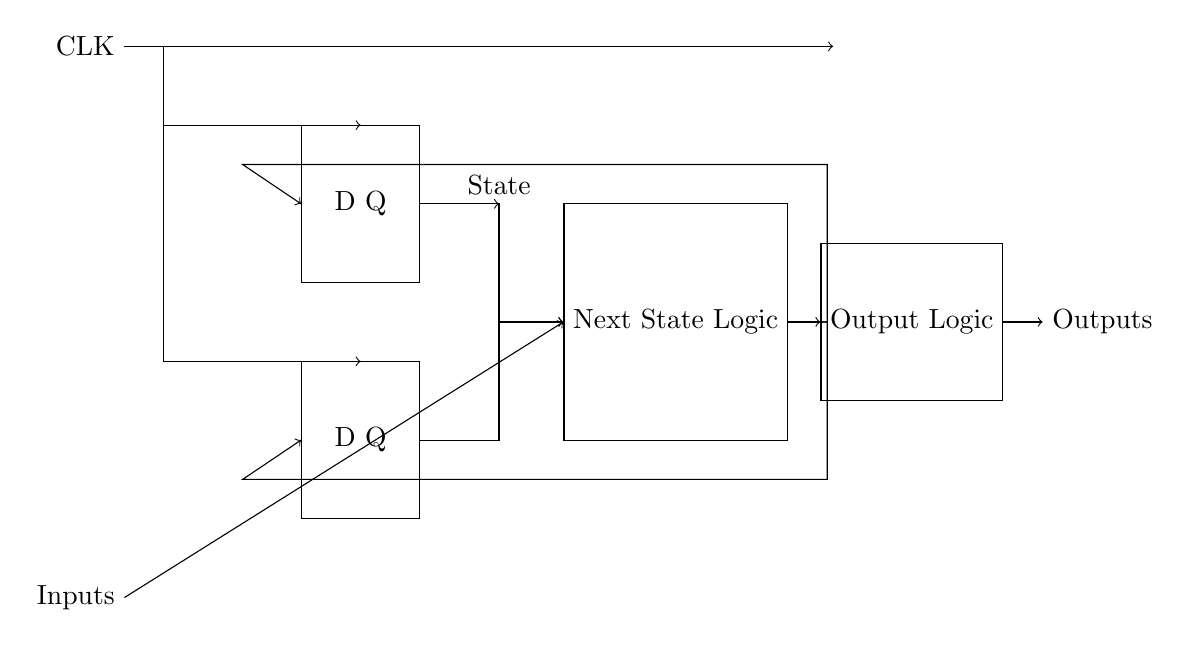
\begin{tikzpicture}[node distance=2cm]
        % Clock
        \draw (0,0) node[left] {CLK} -- (0.5,0);
        \draw[->] (0.5,0) -- (9,0);

        % D Flip-flops
        \node[draw, minimum width=1.5cm, minimum height=2cm] (ff1) at (3,-2) {D Q};
        \node[draw, minimum width=1.5cm, minimum height=2cm] (ff2) at (3,-5) {D Q};

        % Combinational Logic
        \node[draw, minimum width=2cm, minimum height=3cm] (combo1) at (7,-3.5) {Next State Logic};

        % Output Logic
        \node[draw, minimum width=2cm, minimum height=2cm] (out) at (10,-3.5) {Output Logic};

        % Connections
        \draw[->] (ff1.east) -- ++(1,0) |- (combo1.west);
        \draw[->] (ff2.east) -- ++(1,0) |- (combo1.west);
        \draw[->] (combo1.east) -- (out.west);

        % Feedback paths
        \draw[->] (combo1.east) -- ++(0.5,0) |- (8.5,-1.5) -- (1.5,-1.5) -- (ff1.west);
        \draw[->] (combo1.east) -- ++(0.5,0) |- (8.5,-5.5) -- (1.5,-5.5) -- (ff2.west);

        % Clock to flip-flops
        \draw[->] (0.5,0) -- (0.5,-1) -- (3,-1);
        \draw[->] (0.5,-1) -- (0.5,-4) -- (3,-4);

        % External inputs
        \draw[->] (0,-7) node[left] {Inputs} -- (combo1.west);

        % Outputs
        \draw[->] (out.east) -- ++(0.5,0) node[right] {Outputs};

        % State labels
        \draw[->] (ff1.east) -- ++(1,0) node[above] {State};
    \end{tikzpicture}
    \caption{Hardware implementation of a state machine using D flip-flops}
    \label{fig:state_machine_implementation}
\end{figure}

\subsection{Sequential Elements: Flip-Flops and Latches}

The core building blocks of state machines are sequential elements that can store state information. The two primary types are latches and flip-flops.

\subsection*{Latches}

Latches are level-sensitive devices that change their output as long as a control signal (enable) is active. The basic latch types are:

\begin{itemize}
    \item SR Latch (Set-Reset)
    \item D Latch (Data)
\end{itemize}

\begin{figure}[h]
    \centering
    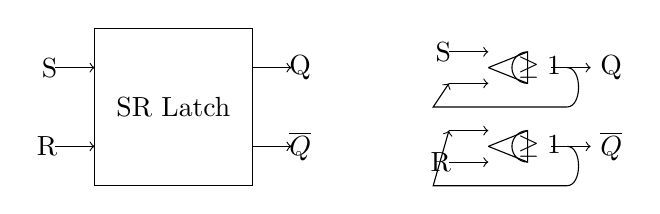
\begin{tikzpicture}
        % SR Latch
        \draw (0,0) rectangle (2,2);
        \node at (1,1) {SR Latch};
        \draw[->] (-0.5,1.5) -- (0,1.5) node[left, pos=0.3] {S};
        \draw[->] (-0.5,0.5) -- (0,0.5) node[left, pos=0.3] {R};
        \draw[->] (2,1.5) -- (2.5,1.5) node[right, pos=0.7] {Q};
        \draw[->] (2,0.5) -- (2.5,0.5) node[right, pos=0.7] {$\overline{Q}$};

        % NOR gate implementation
        \begin{scope}[xshift=5cm]
            % NOR gates
            \draw (0,1.5) -- (0.5,1.7) -- (0.5,1.3) -- (0,1.5);
            \draw (0.5,1.7) arc (90:270:0.2);
            \node at (0.65,1.5) {$\geq 1$};

            \draw (0,0.5) -- (0.5,0.7) -- (0.5,0.3) -- (0,0.5);
            \draw (0.5,0.7) arc (90:270:0.2);
            \node at (0.65,0.5) {$\geq 1$};

            % Connections
            \draw[->] (-0.5,1.7) -- (0,1.7) node[left, pos=0.3] {S};
            \draw[->] (-0.5,1.3) -- (0,1.3);
            \draw[->] (-0.5,0.7) -- (0,0.7);
            \draw[->] (-0.5,0.3) -- (0,0.3) node[left, pos=0.3] {R};

            \draw[->] (0.8,1.5) -- (1.3,1.5) node[right] {Q};
            \draw[->] (0.8,0.5) -- (1.3,0.5) node[right] {$\overline{Q}$};

            % Feedback connections
            \draw[->] (1,1.5) to[out=0,in=0] (1,1) to[out=180,in=0] (-0.7,1) -- (-0.5,1.3);
            \draw[->] (1,0.5) to[out=0,in=0] (1,0) to[out=180,in=0] (-0.7,0) -- (-0.5,0.7);
        \end{scope}
    \end{tikzpicture}
    \caption{SR Latch symbol and implementation using NOR gates}
    \label{fig:sr_latch}
\end{figure}

\subsection*{Flip-Flops}

Flip-flops are edge-triggered devices that change state only at the active edge (rising or falling) of a clock signal. Common types include:

\begin{itemize}
    \item D Flip-Flop
    \item JK Flip-Flop
    \item T Flip-Flop
\end{itemize}

\begin{figure}[h]
    \centering
    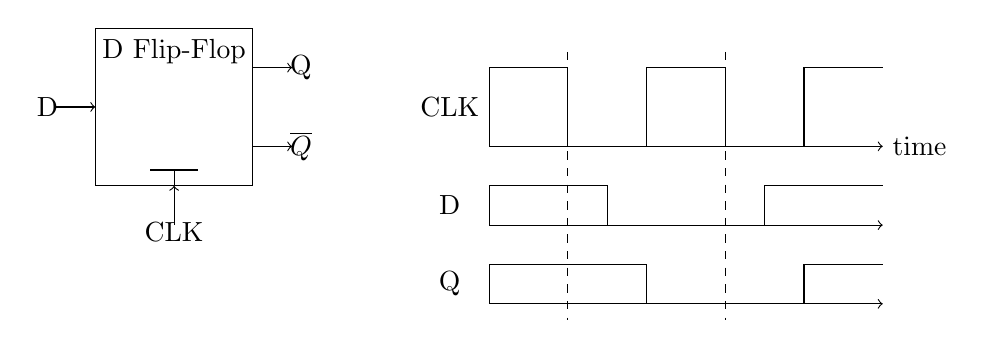
\begin{tikzpicture}[node distance=4cm]
        % D Flip-flop
        \draw (0,0) rectangle (2,2);
        \node at (1,1.7) {D Flip-Flop};
        \draw[->] (-0.5,1) -- (0,1) node[left, pos=0.3] {D};
        \draw[->] (1,-0.5) -- (1,0) node[below, pos=0.3] {CLK};
        \draw (0.7,0.2) -- (1.3,0.2);
        \draw (1,0.2) -- (1,0); % Clock triangle
        \draw[->] (2,1.5) -- (2.5,1.5) node[right, pos=0.7] {Q};
        \draw[->] (2,0.5) -- (2.5,0.5) node[right, pos=0.7] {$\overline{Q}$};

        % Timing diagram
        \begin{scope}[xshift=5cm, yshift=0.5cm]
            % Clock
            \draw[->] (0,0) -- (5,0) node[right] {time};
            \draw (0,0) -- (0,1) -- (1,1) -- (1,0) -- (2,0) -- (2,1) -- (3,1) -- (3,0) -- (4,0) -- (4,1) -- (5,1);
            \node at (-0.5,0.5) {CLK};

            % D input
            \draw[->] (0,-1) -- (5,-1);
            \draw (0,-1) -- (0,-0.5) -- (1.5,-0.5) -- (1.5,-1) -- (3.5,-1) -- (3.5,-0.5) -- (5,-0.5);
            \node at (-0.5,-0.75) {D};

            % Q output
            \draw[->] (0,-2) -- (5,-2);
            \draw (0,-2) -- (0,-1.5) -- (2,-1.5) -- (2,-2) -- (4,-2) -- (4,-1.5) -- (5,-1.5);
            \node at (-0.5,-1.75) {Q};

            % Rising edge indicators
            \draw[dashed] (1,1.2) -- (1,-2.2);
            \draw[dashed] (3,1.2) -- (3,-2.2);
        \end{scope}
    \end{tikzpicture}
    \caption{D Flip-Flop symbol and timing diagram showing edge-triggered behavior}
    \label{fig:d_flipflop}
\end{figure}

\subsection{State Machine Design Methodology}

The design of state machines follows a systematic approach:

\begin{enumerate}
    \item Problem analysis and specification
    \item State diagram creation
    \item State minimization (if necessary)
    \item State encoding
    \item Next-state and output logic derivation
    \item Hardware implementation
    \item Verification and testing
\end{enumerate}

\subsection*{Example: Sequence Detector}

Consider a sequence detector that outputs 1 when it detects the sequence "101" in a serial input stream.

\begin{figure}[h]
    \centering
    \begin{tikzpicture}[node distance=3cm, on grid, auto]
        % States
        \node[state, initial] (S0) {$S_0$};
        \node[state] (S1) [right=of S0] {$S_1$};
        \node[state] (S2) [right=of S1] {$S_2$};
        \node[state] (S3) [below=2cm of S1] {$S_3$};

        % State transitions
        \path[->]
        (S0) edge node {1} (S1)
        (S0) edge [loop above] node {0} ()
        (S1) edge node {0} (S2)
        (S1) edge [loop above] node {1} ()
        (S2) edge [bend left=15] node {1} (S3)
        (S2) edge [bend right=15] node {0} (S0)
        (S3) edge [bend right=45] node[above left] {0,1} (S0);

        % Output labels (Moore machine)
        \node[below=0.2cm] at (S0) {$y=0$};
        \node[below=0.2cm] at (S1) {$y=0$};
        \node[below=0.2cm] at (S2) {$y=0$};
        \node[below=0.2cm] at (S3) {$y=1$};
    \end{tikzpicture}
    \caption{State diagram for a "101" sequence detector implemented as a Moore machine}
    \label{fig:sequence_detector}
\end{figure}

The corresponding state table would be:

\begin{table}[h]
    \centering
    \begin{tabular}{|c|c|c|c|}
        \hline
        \textbf{Current State} & \textbf{Input} & \textbf{Next State} & \textbf{Output} \\
        \hline
        $S_0$                  & 0              & $S_0$               & 0               \\
        $S_0$                  & 1              & $S_1$               & 0               \\
        $S_1$                  & 0              & $S_2$               & 0               \\
        $S_1$                  & 1              & $S_1$               & 0               \\
        $S_2$                  & 0              & $S_0$               & 0               \\
        $S_2$                  & 1              & $S_3$               & 0               \\
        $S_3$                  & 0              & $S_0$               & 1               \\
        $S_3$                  & 1              & $S_0$               & 1               \\
        \hline
    \end{tabular}
    \caption{State transition table for the "101" sequence detector}
    \label{tab:sequence_detector}
\end{table}

\subsection{Special Types of State Machines}

\subsection*{Registers and Counters}

Registers and counters are specialized state machines with specific purposes. A register stores binary information, while a counter progresses through a sequence of states.

\begin{figure}[h]
    \centering
    \begin{tikzpicture}[node distance=2.5cm, on grid, auto]
        % 3-bit counter states
        \node[state, initial] (S0) {000};
        \node[state] (S1) [above right=of S0] {001};
        \node[state] (S2) [below right=of S1] {010};
        \node[state] (S3) [below left=of S2] {011};
        \node[state] (S4) [below left=of S3] {100};
        \node[state] (S5) [below right=of S4] {101};
        \node[state] (S6) [above right=of S5] {110};
        \node[state] (S7) [above left=of S6] {111};

        % Transitions
        \path[->]
        (S0) edge (S1)
        (S1) edge (S2)
        (S2) edge (S3)
        (S3) edge (S4)
        (S4) edge (S5)
        (S5) edge (S6)
        (S6) edge (S7)
        (S7) edge [bend right=45] (S0);
    \end{tikzpicture}
    \caption{State diagram of a 3-bit binary counter}
    \label{fig:binary_counter}
\end{figure}

\subsection*{Finite State Machines with Datapath (FSMD)}

More complex designs combine a state machine controller with a datapath that performs operations on data.

\begin{figure}[h]
    \centering
    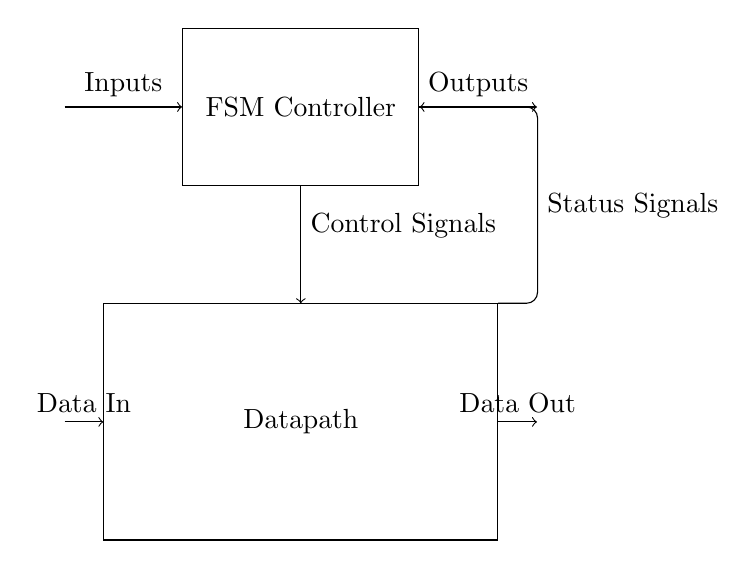
\begin{tikzpicture}
        % Controller
        \node[draw, minimum width=3cm, minimum height=2cm] (controller) at (0,0) {FSM Controller};

        % Datapath
        \node[draw, minimum width=5cm, minimum height=3cm] (datapath) at (0,-4) {Datapath};

        % Connections
        \draw[->, rounded corners] (controller.south) -- ++(0,-0.5) -| (datapath.north) node[pos=0.25, right] {Control Signals};
        \draw[->, rounded corners] (datapath.north east) -- ++(0.5,0) |- (controller.east) node[pos=0.25, right] {Status Signals};

        % External connections
        \draw[->] (-3,0) -- (controller.west) node[midway, above] {Inputs};
        \draw[->] (controller.east) -- (3,0) node[midway, above] {Outputs};
        \draw[->] (-3,-4) -- (datapath.west) node[midway, above] {Data In};
        \draw[->] (datapath.east) -- (3,-4) node[midway, above] {Data Out};
    \end{tikzpicture}
    \caption{Architecture of a Finite State Machine with Datapath (FSMD)}
    \label{fig:fsmd}
\end{figure}